\documentclass[11pt, a4paper, tikz]{article}

\usepackage[english]{babel} %language
\usepackage[utf8]{inputenc} %UTF-8 encoding
\usepackage[margin=0.5in]{geometry} %smaller margin
\usepackage{amssymb} %\nexists \mathbb
\usepackage{amsmath}
\usepackage{amsthm}
\usepackage{graphicx}
\usepackage{polynom}
\usepackage{mathtools}
\usepackage{enumitem}

\usepackage{xlop}
\usepackage[dvipsnames]{xcolor}
\usepackage{tcolorbox}

\definecolor{formulationFrameColor}{RGB}{150,160,190}
\definecolor{formulationBackgroundColor}{RGB}{240,245,250}

\newtcolorbox{formulationBox}{
	colframe=formulationFrameColor,
	colback=formulationBackgroundColor
}

\usepackage{tikz}   
\usepackage{pgfplots}

\pgfplotsset{compat=1.6}

\pgfplotsset{soldot/.style={color=red,only marks,mark=*}} \pgfplotsset{holdot/.style={color=red,fill=white,only marks,mark=*}}

\pgfplotsset{compat=newest} % used to declare my style command.  

\newcommand{\newpara}{
	\vskip 2mm
}

\newcommand{\centsection}[1]{
	\section*{\centering{#1}}
}

\newcommand{\centsubsection}[1]{
	\subsection*{\centering{#1}}
}

\newcommand{\myOver}[2]{
	\ensuremath{\overset{\kern2pt #1}{#2}}
}

\newcommand{\final}[1]{
	$\mathcal{F}($#1$)$
}

\renewcommand{\qed}{\hfill\blacksquare}

\newcommand{\Lim}[1]{\raisebox{0.5ex}{\scalebox{0.8}{$\displaystyle \lim_{#1}\;$}}}
\newcommand{\Inf}[1]{\raisebox{0.5ex}{\scalebox{0.8}{$\displaystyle \inf_{#1}\;$}}}
\newcommand{\Sup}[1]{\raisebox{0.5ex}{\scalebox{0.8}{$\displaystyle \sup_{#1}\;$}}}
\newcommand{\Sum}[2]{\displaystyle \sum_{#1}^{#2}}
\newcommand{\Int}[2]{\displaystyle \int_{#1}^{#2}}

\newcommand{\naturals}{
	\ensuremath{\mathbb{N}}
}
\newcommand{\integers}{
	\ensuremath{\mathbb{Z}}
}
\newcommand{\rationals}{
	\ensuremath{\mathbb{Q}}
}
\newcommand{\reals}{
	\ensuremath{\mathbb{R}}
}
\newcommand{\complexes}{
	\ensuremath{\mathbb{C}}
}

\newcommand{\cover}[1]{
	\ensuremath{\mathcal{#1}}
}

\graphicspath{ {./media/} }

\begin{document}
	\title{\textbf{Chapter 2 — Section A}}
	\maketitle
	%\setcounter{section}{3}
	\centsection{Exercise 1}
	
	\begin{formulationBox}
		Prove that if $A$ and $B$ are subsets of $\reals$ and $|B|=0$, then $|A\cup B| = |A|$.
	\end{formulationBox}
	
	By theorem 2.5, \textit{outer measure preserves order}, as $A$ and $A\cup B$ are subsets of $\reals$ with $A\subseteq A\cup B$, then $|A| \leq |A\cup B|$.
	\newpara
	Now, by theorem 2.8, \textit{countable subadditivity of outer measure}, and as it trivially implies finite subadditivity, we have $|A\cup B| \leq |A| + |B| = |A| + 0 = |A|$.
	\newpara
	As we have both $|A\cup B| \leq |A|$ and $|A| \leq |A\cup B|$, we get $|A\cup B| = |A|$.
	
	$\qed$
	
	\centsection{Exercise 4}
	
	\begin{formulationBox}
		Suppose $F$ is a subset of $\reals$ with the property that every open cover of $F$ has a finite subcover. Prove that $F$ is closed and bounded.
	\end{formulationBox}
	
	Let's first apply some logic rules to look at the problem from a different perspective. The statement \[\textrm{every open cover of $F$ has a finite subcover $\implies$ $F$ is closed and bounded}\] is equivalent to \[\textrm{$F$ is not closed or is unbounded $\implies$ there exists some open cover of $F$ that doesn't have a finite subcover}.\]
	
	Suppose $G$ is an unbounded interval, we can define a cover $\cover{C}=\{(-k, k):k\in\reals^+\}$ that trivially doesn't have a finite subcover for such intervals. Therefore, any unbounded subset of $\reals$ has a cover without a finite subcover.
	
	Now suppose $G$ is an open interval of the form $(a, b)$, with both $a\in\reals$ and $b\in\reals$. Then we can define a cover $\cover{C}=\{(a+\frac{1}{k}, b-\frac{1}{k}):k\in\reals^+\}$ that doesn't have a finite subcover.
	
	For intervals of the form $[a,b)$, we can define a cover $\cover{C}=\{(a-1, b-\frac{1}{k}):k\in\reals^+\}$ that doesn't have a finite subcover. The same idea can be applied for intervals of the form $(a,b]$.
	
	For unions of the previous intervals, we just take into account the supremum and the infimum to define the cover. For example, the cover we define for a subset $G=(a,b)\cup(c,d]$ is $\cover{C} = \{(a+\frac{1}{k}, d+1]:k\in\reals^+\}$.
	
	If the supremum and infimum end points are closed, we can still take advantage of the openness of any other end points in the intervals that constitute the subset. For example, we could define the following cover for a subset $G=[a,b)\cup[c,d)\cup[e,f]$: $\cover{C}=\{(a-1,b-\frac{1}{k})\cup(c-\epsilon,f+1):k\in\reals^+\}$, with $\epsilon>0$ such that the subintervals do not intersect with each other.
	
	We have proved that for any unbounded or non-closed subset $G$ of $\reals$ there exists some cover $\cover{C}$ that doesn't have a finite subcover. Hence, if a subset of $\reals$ has the property that all of its open covers have a finite subcover, then that subset must be closed and bounded.
	
	$\qed$
	
	\centsection{Exercise 6}
	
	\begin{formulationBox}
		Prove that if $a,b\in\reals$ and $a<b$, then \[|(a,b)| = |[a,b)| = |(a,b]| = b-a.\]
	\end{formulationBox}
	
	By theorem 2.14, \textit{outer measure of a closed interval}, $|[a,b]| = b-a$.
	
	We know $[a,b] = (a,b)\cup\{a,b\}$. Since $\{a,b\}$ is a countable set, $|\{a,b\}| = 0$. By the theorem proved in exercise 1, $|(a,b)| = |(a,b)\cup\{a,b\}| = |[a,b]| = b-a$.
	
	We replace $\{a,b\}$ with $\{a\}$ or $\{b\}$ to prove for $(a,b]$ and $[a,b)$ respectively.
	
	$\qed$
	
	\centsection{Exercise 9}
	
	\begin{formulationBox}
		Prove that $|A| = \Lim{t\rightarrow\infty}|A\cap(-t,t)|$ for all $A\subseteq\reals$.
	\end{formulationBox}
	
	For any $x\in\reals$, we can find some $t\in\reals$ (namely $t=|x|$) such that $x\in(-T,T)\ \forall T\geq t$. This, in essence, means that $\Lim{t\rightarrow\infty}(-t,t) = \reals$.
	
	Therefore, the intersection in the expression given to us will contain all elements in $A$ for big enough values of $t$, so the intersection will equal $A$ and, therefore, their outer measures will be the same.
	
	$\qed$
	
	\centsection{Exercise 10}
	
	\begin{formulationBox}
		Prove that $|[0,1]\setminus\rationals| = 1$.
	\end{formulationBox}
	
	We know, since $\rationals$ is a countable set, that $|\rationals| = 0$. Then, by the theoren proved in exercise 1, $|[0,1]\setminus\rationals| = |([0,1]\setminus\rationals) \cup \rationals| = |[0,1]| = 1-0 = 1$.
	
	$\qed$
		
	\centsection{Exercise 14}
	
	\begin{formulationBox}
		Consider the following figure, which is drawn accurately to scale.
		
		\centering{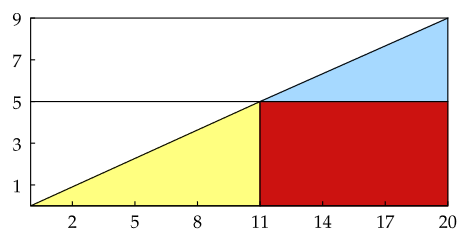
\includegraphics[scale=0.7]{./2A-14-1}}
		
		\begin{enumerate}[label=\alph*)]
			\item Show that the right triangle whose vertices are $(0,0)$, $(20, 0)$ and $(20, 9)$ has area $90$.
			\item Show that the yellow (lower) right triangle has area $27.5$.
			\item Show that the red rectangle has area $45$.
			\item Show that the blue (upper) right triangle has area $18$.
			\item Add the results of parts b), c) and d), showing that the area of the colored region is $90.5$.
			\item Explain why the results obtained in a) and e) differ.
		\end{enumerate}
	\end{formulationBox}

	\begin{enumerate}[label=\alph*)]
		\item Such triangle has height $9-0=9$ and width $20-0=20$, so its area is $\frac{20\cdot9}{2} = 90$.
		\item Similarly, the area of the yellow triangle is $\frac{(11-0)(5-0)}{2} = 27.5$.
		\item The area of the red rectangle is $(20-11)(5-0) = 45$.
		\item The area of the blue triangle has area $\frac{(20-11)(9-5)}{2} = 18$.
		\item The area of the colored region is $27.5 + 45 + 18 = 90.5$.
		\item The colored region is actually not a triangle, just a right trapezoid with an angle very close to $180^\circ$. The triangle described in part a) has a slope of $\frac{9}{20}$, while the yellow and blue triangles have slopes $\frac{5}{11}$ and $\frac{4}{9}$ respectively. The following picture illustrates that there is indeed a separation between the lines, although it is hard to see without zooming in.
		
		\centering{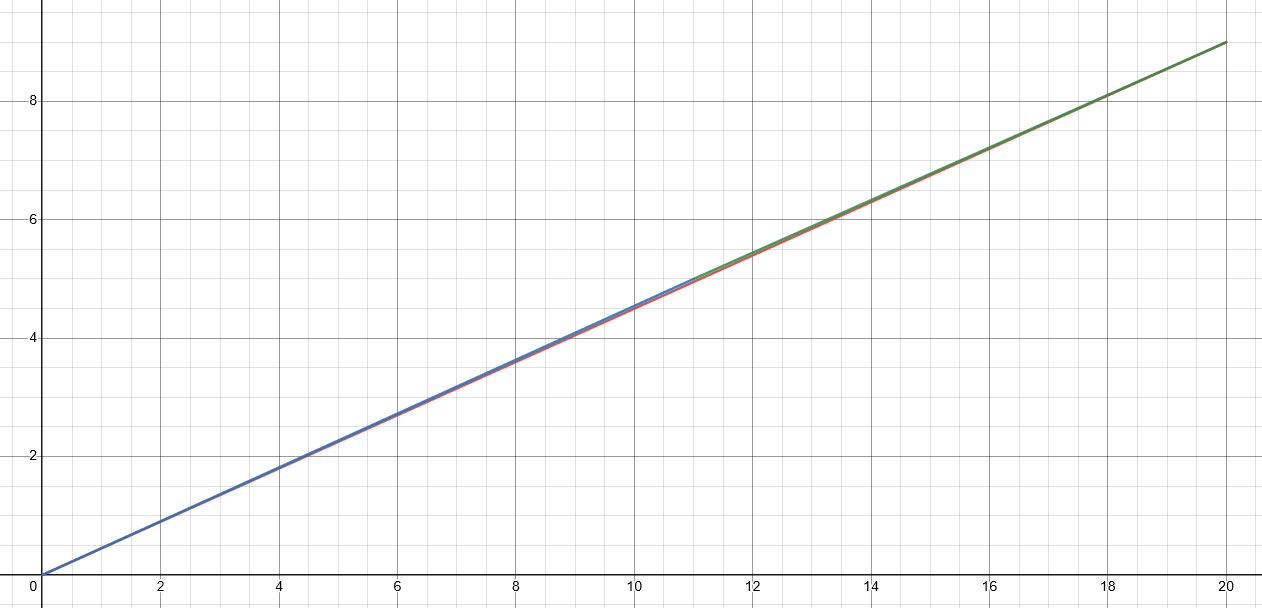
\includegraphics[scale=0.4]{./2A-14-2}}
	\end{enumerate}
	
	I kind of feel like this exercise was a bit off-topic, as in it has nothing to do with the new concepts learned in this chapter.
\end{document}